% Author: Izaak Neutelings (September 2020)
\documentclass[border=3pt,tikz]{standalone}
\usepackage{amsmath}
\usepackage{tikz}
\usepackage{physics}
\usetikzlibrary{intersections}
\usetikzlibrary{decorations.markings}
\usetikzlibrary{angles,quotes} % for pic
\usetikzlibrary{decorations.pathmorphing} % for decorate random steps
\tikzset{>=latex} % for LaTeX arrow head
\usepackage{xcolor}
\colorlet{xcol}{blue!70!black}
\colorlet{xcol'}{xcol!50!red!80!black}
\colorlet{veccol}{green!45!black}
\tikzstyle{vector}=[->,thick,veccol,line cap=round]
\tikzstyle{rvec}=[->,thick,xcol,line cap=round]


\begin{document}

% LAB & COM FRAMES
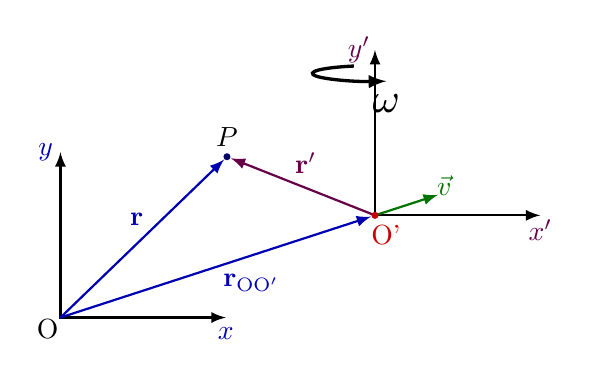
\begin{tikzpicture}
    \def\L{2.1}
    \def\ang{18} % angle of the CM velocity
    \coordinate (O) at (0,0);
    \coordinate (O') at (\ang:2.0*\L);
    \coordinate (R) at (44:1.4*\L);
    \node[fill=blue!40!black,circle,inner sep=0.9] (R') at (R) {};
    \node[above] at (R) {$P$};
    % LAB
    \draw[<->,thick] (\L,0) node[below,xcol] {$x$} -- (O) node[below left=-3] {O} -- (0,\L) node[left=-1,xcol] {$y$};
    \draw[rvec] (O) -- (R') node[midway,left=2,above=1] {$\vb{r}$}; %$(\vb{r})_\mathrm{lab}$
    \draw[<->,thick] (O')++(\L,0) node[below=-2,xcol'] {$x'$} --++ (-\L,0) node[red!80!black,right=4,below] {O'} --++ (0,\L) node[left=-2,xcol'] {$y'$};
    \draw[rvec,xcol'] (O') -- (R') node[midway,right=1,above=1] {$\vb{r}'$}; %(\vb{r})_\mathrm{cm}
    \draw[vector] (O') --++ (\ang:0.4*\L) node[above right=-4] {$\vec{v}$}; %(\vb{v}_\mathrm{cm})_\mathrm{lab}
    \node[fill=red!80!black,circle,inner sep=0.9] (CM) at (O') {};
    \draw[rvec] (O) -- (CM) node[midway,below right=-1] {$\vb{r}_\mathrm{OO'}$}; %(\vb{r}_\mathrm{cm})_\mathrm{lab}
    \draw[->,very thick,rotate=0] (4,\L+1)++(-250:{0.8} and {0.1}) arc (-250:-80:{0.8} and {0.1}) node[below=-1,scale=1.5] {$\omega$};
\end{tikzpicture}

\end{document}